% QUESTAO
A figura abaixo é composta de cinco quadrados de lado $a$.
\begin{center}
	\vspace{-3mm}
	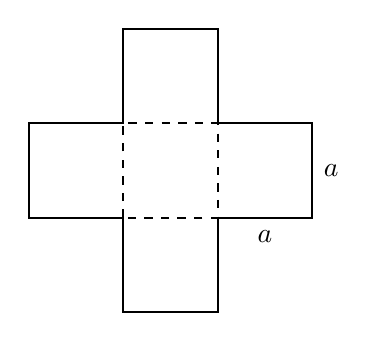
\begin{tikzpicture}[scale=1.2]
	\draw[thick] (0,0)--(-1,0)--(-1,1)--(0,1)--(0,2)--(1,2)--(1,1)--(2,1)--(2,0)--(1,0)--(1,-1)--(0,-1)--cycle;
	\draw[thick,dashed] (0,0) rectangle (1,1);
	\node at (1.5,-0.2) {$a$};
	\node at (2.2,0.5) {$a$};
	\end{tikzpicture}
	\vspace{-3mm}
\end{center}
Quais as expressões algébricas que representam a área $(A)$ e o perímetro $(P)$ dessa figura?

% ALTERNATIVAS 7
$A=5a^2$ e $P=12a$
$A=4a^2$ e $P=14a^2$
$A=3a^3$ e $P=16a$
$A=2a^5$ e $P=18a^4$
$A=a^2$ e $P=20a$



